% BEGIN PREAMBEL
\documentclass[9pt]{beamer}
\usepackage[british]{babel}
\usepackage[latin1]{inputenc}
\usepackage{multimedia}
\usepackage{amsmath,amsfonts,amssymb}
\usepackage{upgreek}
\usepackage{pgfpages}
\usepackage[version=3]{mhchem}
\usepackage{lmodern}
\usepackage{graphicx}
\usepackage{multicol}
\usepackage{color}
\usepackage{xcolor}
\usepackage{wrapfig}
\usepackage{siunitx}
\usepackage{fontspec}
\newfontfamily\ubuntu{Ubuntu}
\newcommand{\as}{\\[14pt]}
\newcommand{\s}{\\[7pt]}
\newcommand{\is}{\\[2pt]}
\newcommand{\no}{\noindent}
\newcommand{\ka}{\hspace*{0.5cm}}
\newcommand{\ma}{\hspace*{1cm}}
\newcommand{\ga}{\hspace*{1.5cm}}
\newcommand{\li}{\left|}
\newcommand{\re}{\right|}
\newcommand{\const}{\text{const.}}
\newcommand{\z}{\text}
\newcommand{\terminal}[1]{\colorbox{black}{\textcolor{white}{{\fontfamily{phv}\selectfont \scriptsize{#1}}}}}
\newcommand{\plugin}[1]{\textit{\flq#1\frq}}
\usetheme{Boadilla}
\graphicspath{ {Pics/} }
\usecolortheme{beaver}
\useoutertheme{miniframes}
\beamertemplatenavigationsymbolsempty
\makeindex
\title[Pad Performance]{Diamond pad detector performance at high rate at PSI}
\author[M. Reichmann]{Michael Reichmann}
\institute[\textbf{\textit{ETH}}\scalebox{.6}{\textit{Z\"{u}rich}}]{Swiss Federal Institute of Technology Zurich}
% END PREAMBEL
\begin{document}
% ============================
% BEGIN TITLE PAGE
% ============================
\begin{frame}
	\begin{center}
		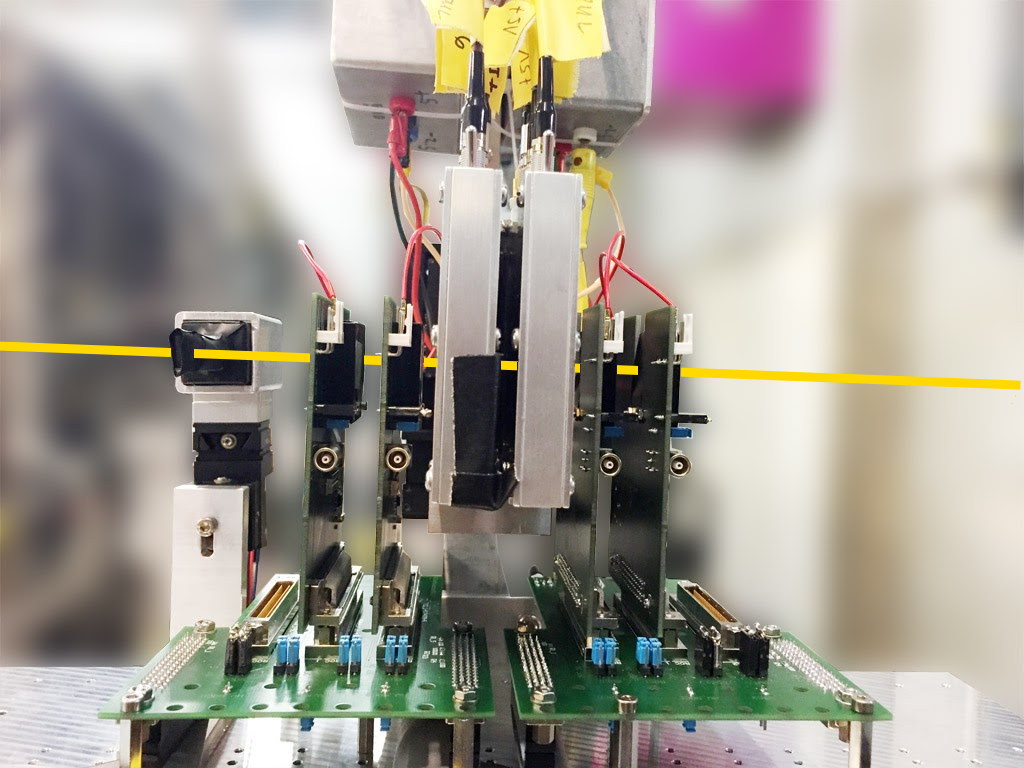
\includegraphics[width=6cm]{Setup1}
	\end{center}
	\begin{alertblock}{
		\begin{center}
			\textbf{Diamond pad detector performance at high rate at PSI}
		\end{center}}
		\vspace*{10pt}
		\begin{center}\small
		Michael Reichmann
		\end{center}\normalsize
	\end{alertblock}
\end{frame}
% END
% ============================
% BEGIN TABLE OF CONTENTS
% ============================
\begin{frame}[allowframebreaks]
	\frametitle{Table of contents}
	\tableofcontents   % [pausesections]
\end{frame}
% END
% ====================================================================================
% INTRODUCTION
% ====================================================================================
\section{Introduction}
% ============================
\begin{frame}
	\underline{\textbf{Goal:}}
	\begin{itemize}
		\item investigate if polychrystalline diamond pad detectors show a rate dependent pulse height
	\end{itemize}
	\vspace*{1cm}
	\underline{\textbf{Measurements:}}
	\begin{itemize}
		\setlength{\itemsep}{\fill}
		\item tests of several diamonds pad detectors with a \SI{250}{Mev/c} pion beam at PSI
		\item brands:
		\begin{itemize}
			\item Element 6
			\item .$\hdots$
		\end{itemize}
		\item rate range: from \SI{1}{kHz/cm^{2}} up to \SI{10}{MHz/cm^{2}}
	\end{itemize}
\end{frame}
% new frame ==================
\begin{frame}
	\frametitle{Setup}
	\begin{center}
		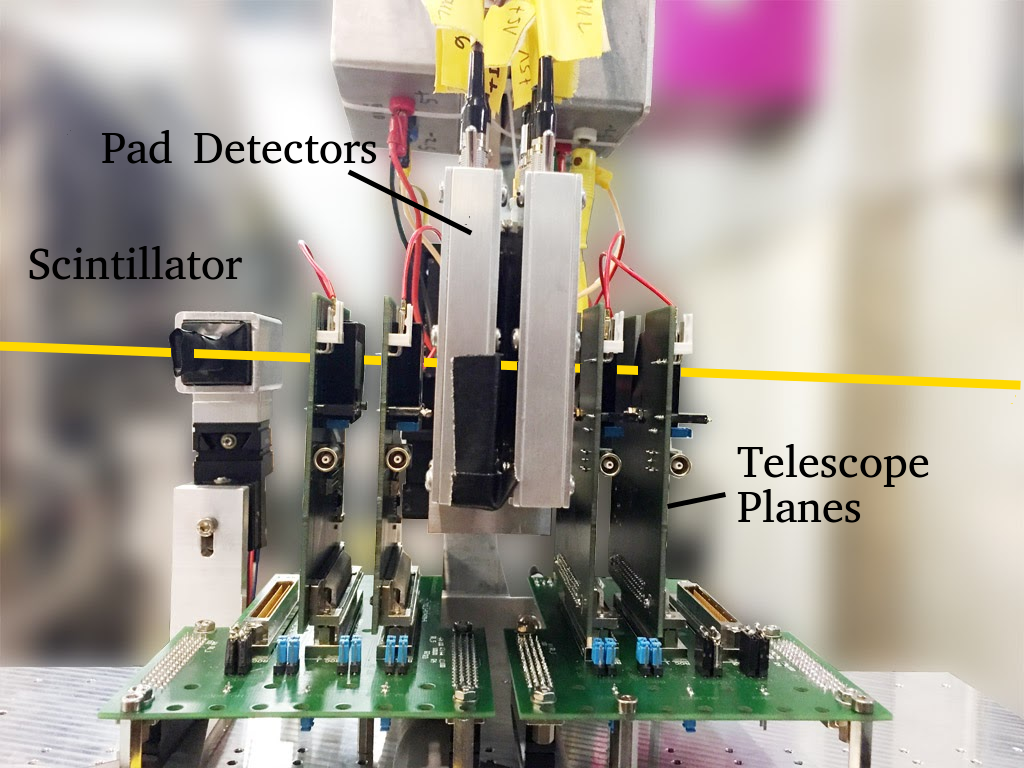
\includegraphics[width=6cm]{Setup}
	\end{center}
	\begin{itemize}
		\setlength{\itemsep}{\fill}
		\item 4 tracking planes with analogue CMS pixel chips
		\item 2 diamond pad detectors
		\item scintillator for precise timing
	\end{itemize}
\end{frame}
% ====================================================================================
% ANALYSIS
% ====================================================================================
\section{Analysis}
% ============================
\begin{frame}
	bla
\end{frame}
% ====================================================================================
% INTRODUCTION
% ====================================================================================
\section{Results}
% ============================
\begin{frame}
	bla
\end{frame}
% ====================================================================================
% CONCLUSION
% ====================================================================================
\section{Conclusion}
% ============================
\begin{frame}
	\frametitle{Conclusion}
	\begin{itemize}
		\item tested several diamond pad detectors with fluxes between \SI{1}{kHz/cm^{2}} and \SI{10}{MHz/cm^{2}}
		\item some of the diamond pad detectors have only a very slight ($1-3$\%) rate dependence after irradiation
	\end{itemize}
\end{frame}
% ============================
% DOCUMENT END
\end{document}

